\chapter{Hồi quy động học và ma trận hiệp phương sai}
\section{Thuật toán hồi quy và trích xuất ma trận hiệp phương sai}
\label{sec:theory_pcov}

Trong phân tích dữ liệu thực nghiệm tự động hóa, sau khi các mảng dữ liệu thô được nạp từ các tệp lưu trữ ngoại vi (như định dạng \texttt{.csv}), việc ước lượng các hằng số vật lý cốt lõi (như gia tốc trọng trường $g$) đòi hỏi việc khớp dữ liệu đo với các mô hình toán học. Đối với hệ thống lấy mẫu tự động, dữ liệu đầu vào mang những mức độ bất định hệ thống nhất định. Do đó, quá trình khớp đường cong (curve fitting) không chỉ nhằm mục đích ước lượng quỹ đạo trung tâm, mà còn đóng vai trò ước lượng độ bất định của các tham số thông qua ma trận hiệp phương sai.

\begin{physcore}{Nguyên lý tối ưu hóa bình phương tối thiểu trọng số}{weighted_least_squares}
Hàm tối ưu hóa hồi quy phi tuyến trong các thư viện phân tích khoa học vận hành dựa trên nguyên lý bình phương tối thiểu trọng số (weighted least squares). Đối với tập dữ liệu động học có chứa phương sai đo lường $\sigma_i^2$, thuật toán tiến hành cực tiểu hóa hàm tổng bình phương phần dư được chuẩn hóa $S(\theta)$:
\begin{equation}
    S(\theta) = \sum_{i=1}^{N} \left[ \frac{y_i - f(x_i, \theta)}{\sigma_i} \right]^2 \label{eq:weighted_least_squares}
\end{equation}
Trong đó, $f(x_i, \theta)$ biểu thị mô hình lý thuyết (hàm bậc hai đối với tọa độ hoặc hàm tuyến tính đối với vận tốc). Việc sử dụng trọng số nghịch đảo $1/\sigma_i$ đảm bảo rằng các điểm dữ liệu sở hữu độ bất định cao sẽ có mức độ đóng góp thấp hơn vào quá trình ảnh hưởng đến kết quả hồi quy, từ đó phản ánh đúng mức độ tin cậy của từng điểm đo.
\end{physcore}

Quá trình giải bài toán cực trị bằng các thuật toán lặp đa chiều (như thuật toán Levenberg-Marquardt) sẽ trả về bộ tham số tối ưu (optimal parameters) và ma trận hiệp phương sai (covariance matrix). Ma trận này, thường được định danh là biến \texttt{pcov} trong môi trường lập trình, đóng vai trò là cơ sở cho việc phân tích sai số cho các phép đo gián tiếp.

\begin{derivation}{Cấu trúc giải tích của ma trận hiệp phương sai}{cov_matrix_structure}
Ma trận hiệp phương sai $\Sigma$ (tương ứng đối tượng \texttt{pcov}) cho một mô hình có $M$ tham số tự do là một ma trận vuông đối xứng cấp $M$. Thông tin về độ bất định và tương quan sai số được thể hiện qua các phần tử:
\begin{equation}
    \Sigma = \begin{pmatrix}
    \sigma_{1}^2 & \text{cov}_{1,2} & \cdots & \text{cov}_{1,M} \\
    \text{cov}_{2,1} & \sigma_{2}^2 & \cdots & \text{cov}_{2,M} \\
    \vdots  & \vdots  & \ddots & \vdots  \\
    \text{cov}_{M,1} & \text{cov}_{M,2} & \cdots & \sigma_{M}^2
    \end{pmatrix} \label{eq:covariance_matrix}
\end{equation}
Trong đó, phần tử trên đường chéo chính $\Sigma_{ii} = \sigma_i^2$ là phương sai (variance) của tham số hồi quy thứ $i$. Độ lệch chuẩn tuyệt đối của tham số (ví dụ: gia tốc trọng trường $g$) được tính bằng căn bậc hai của phần tử đường chéo tương ứng:
\begin{equation}
    u_{\theta_i} = \sqrt{\Sigma_{ii}} \label{eq:std_dev_extraction}
\end{equation}
Các phần tử ngoài đường chéo $\Sigma_{ij}$ biểu thị mức độ tương quan hiệp phương sai (covariance) giữa các đại lượng.
\end{derivation}

Thư viện \texttt{scipy.optimize} cung cấp hàm \texttt{curve\_fit} để tự động hóa thuật toán trên. Khi áp dụng vào bài toán minh họa rơi tự do, phương trình $s(t) = 0.5gt^2 + v_0t + s_0$ được viết dưới dạng hàm Python. Trọng số sai số được tích hợp trực tiếp thông qua đối số \texttt{sigma}. Các phần tử trên đường chéo ma trận được trích xuất tự động qua các hàm tính toán mảng (vectorized operations) của thư viện \texttt{numpy}.

\begin{pycode}{Kinematic regression and covariance matrix extraction}
from scipy.optimize import curve_fit

# Define Theoretical Models for Free Fall Kinematics
def quadratic_displacement_model(t, g, v0, s0):
    # s(t) = 0.5 * g * t^2 + v0 * t + s0
    return 0.5 * g * t**2 + v0 * t + s0

def linear_velocity_model(t, g, v0):
    # v(t) = g * t + v0
    return g * t + v0

# Execute non-linear curve fitting for Displacement data
popt_s, pcov_s = curve_fit(
    quadratic_displacement_model,
    time_data,
    displacement_data,
    sigma=np.full_like(displacement_data, sigma_s),
    absolute_sigma=True,
    p0=[9.8, 0.0, 0.0]
)

# Extract optimized parameters and their absolute standard deviations
g_s_opt, v0_s_opt, s0_opt = popt_s
g_s_err = np.sqrt(np.diag(pcov_s))[0]
\end{pycode}

% \begin{figure}[htbp]
%     \centering
%     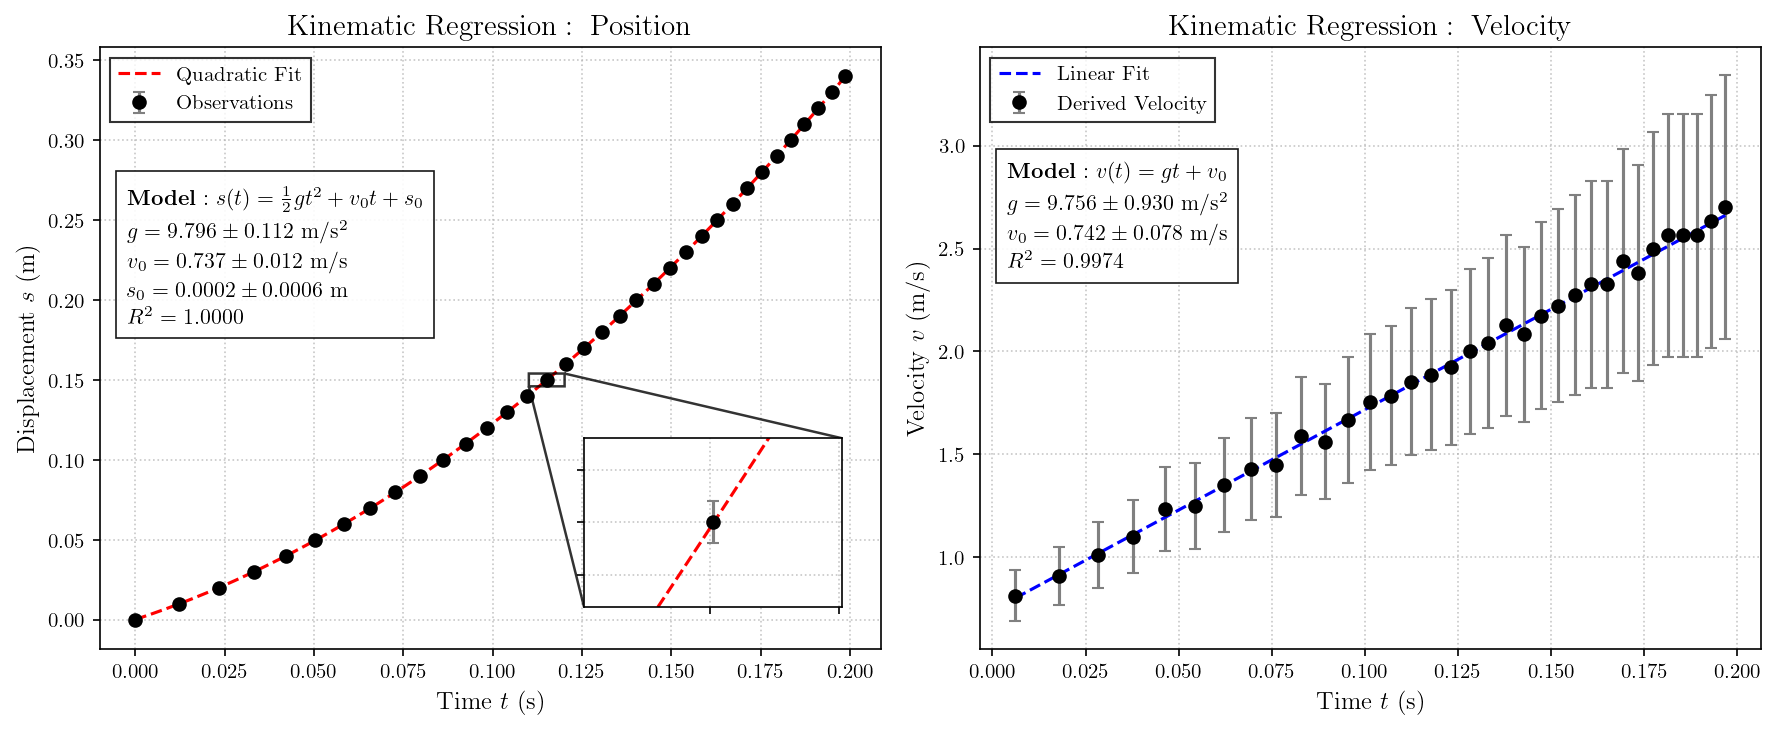
\includegraphics[width=\textwidth]{figures/fig_regression_kinematics.png}
%     \caption{Trực quan hóa đồ thị hồi quy động học và phân bố tham số mô hình từ kết quả phân tích hiệp phương sai.}
%     \label{fig:regression_kinematics}
% \end{figure}

% \begin{pitfall}{Sai lệch cấu trúc sai số do bỏ qua cờ trạng thái absolute\_sigma}{missing_absolute_sigma}
\begin{pitfall}{Sai lệch ma trận hiệp phương sai khi bỏ qua đối số sai số tuyệt đối}{missing_absolute_sigma}
Khi cấu hình \texttt{curve\_fit} cần chú ý rằng sai lệch ước lượng độ bất định nếu bỏ sót tham số \texttt{absolute\_sigma=True}. Mặc định, hàm này giả định các giá trị trong mảng \texttt{sigma} chỉ mang ý nghĩa trọng số tương đối và tiến hành chuẩn hóa ma trận hiệp phương sai dựa trên phương sai của phần dư. Đối với dữ liệu lấy mẫu từ cảm biến, đại lượng độ bất định (như \texttt{sigma\_s}) phản ánh giới hạn độ phân giải vật lý thực tế của thiết bị. Việc không kích hoạt \texttt{absolute\_sigma=True} sẽ khiến kết quả sai số không còn phản ánh đúng giới hạn thiết bị, khiến độ lệch chuẩn được trích xuất từ \texttt{pcov\_s} không còn tương ứng với sai số thực của thiết bị của thiết bị phần cứng.
\end{pitfall}